\section{Evaluation}
\label{sec:evaluation}

\begin{enumerate}
    \item Benchmarks (describe our benchmarks)
    \item Results (total time, split out SMPT time from our rust code time)
    \item Analysis of optimizations (how much time they save, petri net sizes, semilinear set sizes)
    \item Limitations (examples we cannot solve, future work that would help)
\end{enumerate}





\begin{table}[ht]
	\centering
	\resizebox{\textwidth}{!}{%
		\begin{tabular}{%
				l   % Category
				l   % Benchmark
				p{5cm}   % Description
				cccc  % Features: If, While, ?, Yield
				rr    % Runtime: w/ SMPT, w/o SMPT
				c     % Serializable
			}
			\toprule
			\textbf{Category}
			& \textbf{Benchmark}
			& \textbf{Description}
			& \multicolumn{4}{c}{\textbf{Features}}
			& \multicolumn{2}{c}{\textbf{Runtime (ms)}}
			& \textbf{Serializable} \\
			\cmidrule(lr){4-7} \cmidrule(lr){8-9}
			& 
			& 
			& \textbf{If}
			& \textbf{While}
			& \textbf{?}
			& \textbf{Yield}
			& \textbf{w/ SMPT}
			& \textbf{w/o SMPT}
			&  \\
			\midrule
			
			%% Cluster 1: Core expressions & operators
			\multirow{18}{*}{Core expressions \& operators}
			& \texttt{arithmetic.ser}
			& \multirow{18}{5cm}{Benchmarks testing arithmetic, boolean, and simple control expressions}
			&  &  &  & \cmark & -- & -- & \cmark \\
			& \texttt{boolean\_ops.ser}
			& 
			& \cmark &  &  & \cmark & -- & -- & \cmark \\
			& \texttt{seq\_expr.ser}
			& 
			&  &  &  & \cmark & -- & -- & \cmark \\
			& \texttt{multiple\_vars.ser}
			& 
			&  &  &  &  & -- & -- & \cmark \\
			& \texttt{mixed\_expr.ser}
			& 
			& \cmark &  &  &  & -- & -- & \cmark \\
			& \texttt{complex\_expr.ser}
			& 
			& \cmark &  &  &  & -- & -- & \cmark \\
			& \texttt{if\_expr.ser}
			& 
			& \cmark &  &  &  & -- & -- & \cmark \\
			& \texttt{while\_expr.ser}
			& 
			&  & \cmark &  &  & -- & -- & \cmark \\
			& \texttt{if\_while.ser}
			& 
			& \cmark & \cmark &  & \cmark & -- & -- & \cmark \\
			& \texttt{nested\_while.ser}
			& 
			&  & \cmark &  &  & -- & -- & \cmark \\
			& \texttt{ex.ser}
			& 
			&  & \cmark &  & \cmark & -- & -- & \cmark \\
			& \texttt{simple\_assign.ser}
			& 
			&  &  &  &  & -- & -- & \cmark \\
			& \texttt{yield\_expr.ser}
			& 
			&  &  &  & \cmark & -- & -- & \cmark \\
			& \texttt{equality\_check.ser}
			& 
			& \cmark &  &  &  & -- & -- & \cmark \\
			& \texttt{globals.ser}
			& 
			& \cmark &  &  & \cmark & -- & -- & \cmark \\
			& \texttt{with\_comments.ser}
			& 
			&  &  &  & \cmark & -- & -- & \cmark \\
			& \texttt{simple\_nonser2.ser}
			& 
			&  &  &  &  & -- & -- &  \\
			& \texttt{simple\_nonser2\_minus\_yields\_is\_ser.ser}
			& 
			&  &  &  &  & -- & -- &  \\
			\midrule
			
			%% Cluster 2: Fred (mixed arithmetic)
			\multirow{10}{*}{Fred (mixed arithmetic)}
			& \texttt{fred.ser}
			& \multirow{10}{5cm}{Mixed control and arithmetic transformations (Fred series)}
			& \cmark & \cmark &  & \cmark & -- & -- & \cmark \\
			& \texttt{fred2.ser}
			& 
			& \cmark & \cmark &  & \cmark & -- & -- & \cmark \\
			& \texttt{fred2\_arith.ser}
			& 
			&  & \cmark &  & \cmark & -- & -- & \cmark \\
			& \texttt{fred\_arith.ser}
			& 
			&  & \cmark &  & \cmark & -- & -- & \cmark \\
			& \texttt{fred\_arith\_simplified\_until\_1.ser}
			& 
			&  & \cmark &  & \cmark & -- & -- & \cmark \\
			& \texttt{fred\_arith\_simplified\_until\_2.ser}
			& 
			&  & \cmark &  & \cmark & -- & -- & \cmark \\
			& \texttt{fred\_arith\_tricky.ser}
			& 
			&  & \cmark &  & \cmark & -- & -- & \cmark \\
			& \texttt{fred\_arith\_tricky2.ser}
			& 
			&  & \cmark &  & \cmark & -- & -- & \cmark \\
			& \texttt{fred\_arith\_tricky3.ser}
			& 
			&  & \cmark &  & \cmark & -- & -- & \cmark \\
			& \texttt{incrdecr.ser}
			& 
			&  & \cmark &  &  & -- & -- & \cmark \\
			\midrule
			
			%% Cluster 3: Stop (circular-increment) series
			\multirow{7}{*}{Stop (circular-increment) series}
			& \texttt{stop.ser}
			& \multirow{7}{5cm}{Circular increment loops and variants}
			&  & \cmark &  &  & -- & -- & \cmark \\
			& \texttt{stop2.ser}
			& 
			&  & \cmark &  &  & -- & -- & \cmark \\
			& \texttt{stop3.ser}
			& 
			&  &  &  &  & -- & -- & \cmark \\
			& \texttt{stop3a.ser}
			& 
			&  &  &  &  & -- & -- & \cmark \\
			& \texttt{stop4.ser}
			& 
			&  & \cmark &  &  & -- & -- & \cmark \\
			& \texttt{stop4a.ser}
			& 
			&  & \cmark &  &  & -- & -- & \cmark \\
			& \texttt{funny.ser}
			& 
			&  &  &  & \cmark & -- & -- & \cmark \\
			\midrule
			
			%% Cluster 4: Concurrency & locking loops
			\multirow{6}{*}{Concurrency \& locking loops}
			& \texttt{tricky2.ser}
			& \multirow{6}{5cm}{Concurrent looping patterns with locking and tricky interactions}
			&  &  &  &  & -- & -- & \cmark \\
			& \texttt{tricky3.ser}
			& 
			&  &  &  &  & -- & -- & \cmark \\
			& \texttt{tricky3\_ser.ser}
			& 
			&  &  &  &  & -- & -- & \cmark \\
			& \texttt{self\_loop.ser}
			& 
			& \cmark & \cmark &  & \cmark & -- & -- & \cmark \\
			& \texttt{self\_loop2.ser}
			& 
			& \cmark & \cmark &  & \cmark & -- & -- & \cmark \\
			& \texttt{simple\_nonser2\_turned\_ser\_with\_locks.ser}
			& 
			&  &  &  &  & -- & -- &  \\
			\midrule
			
			%% Cluster 5: Non-deterministic choice & randomness
			\multirow{8}{*}{Non-deterministic choice \& randomness}
			& \texttt{nondet.ser}
			& \multirow{8}{5cm}{Random choice and non-deterministic branching benchmarks}
			&  &  & \cmark &  & -- & -- & \cmark \\
			& \texttt{nondet2.ser}
			& 
			&  &  & \cmark &  & -- & -- & \cmark \\
			& \texttt{nondet\_impl.ser}
			& 
			&  &  & \cmark &  & -- & -- & \cmark \\
			& \texttt{nondet\_impl2.ser}
			& 
			&  &  & \cmark & \cmark & -- & -- & \cmark \\
			& \texttt{modulo\_nonser.ser}
			& 
			&  &  & \cmark &  & -- & -- &  \\
			& \texttt{simple\_nonser3.ser}
			& 
			&  &  &  &  & -- & -- &  \\
			& \texttt{flag\_non\_ser.ser}
			& 
			&  &  & \cmark &  & -- & -- &  \\
			& \texttt{flag\_non\_ser\_turned\_ser.ser}
			& 
			&  &  & \cmark &  & -- & -- &  \\
			\midrule
			
			%% Cluster 6: Networking & system protocols
			\multirow{4}{*}{Networking \& system protocols}
			& \texttt{BGP\_routing.ser}
			& \multirow{4}{5cm}{Networking protocols and system-level monitoring}
			& \cmark & \cmark & \cmark & \cmark & -- & -- & \cmark \\
			& \texttt{snapshot\_isolation\_network\_monitoring.ser}
			& 
			& \cmark & \cmark & \cmark & \cmark & -- & -- & \cmark \\
			& \texttt{stateful\_firewall.ser}
			& 
			& \cmark &  & \cmark & \cmark & -- & -- & \cmark \\
			& \texttt{stateful\_firewall\_without\_yields.ser}
			& 
			& \cmark &  & \cmark &  & -- & -- & \cmark \\
			\midrule
			
			%% Cluster 7: Multi-request workflows
			\multirow{4}{*}{Multi-request workflows}
			& \texttt{multiple\_requests.ser}
			& \multirow{4}{5cm}{Benchmarks modelling multiple requests or sequential interactions}
			&  &  &  &  & -- & -- & \cmark \\
			& \texttt{less\_simple\_ser.ser}
			& 
			&  & \cmark &  & \cmark & -- & -- &  \\
			& \texttt{simple\_nonser.ser}
			& 
			&  &  &  &  & -- & -- &  \\
			& \texttt{simple\_ser.ser}
			& 
			&  &  &  & \cmark & -- & -- & \cmark \\
			\midrule
			
			%% Cluster 8: JSON state-machine examples
			\multirow{4}{*}{JSON state-machine examples}
			& \texttt{data\_flow.json}
			& \multirow{4}{5cm}{Example JSON-encoded state machine workflows}
			&  &  &  &  & -- & -- &  \\
			& \texttt{shopping\_cart.json}
			& 
			&  &  &  &  & -- & -- &  \\
			& \texttt{login\_flow.json}
			& 
			&  &  &  &  & -- & -- &  \\
			& \texttt{state\_machine.json}
			& 
			&  &  &  &  & -- & -- &  \\
			
			\bottomrule
		\end{tabular}%
	}
	\caption{Overview of all benchmarks by category, features, runtime, and serializability.}
	\label{tab:benchmarks}
\end{table}


\begin{figure}[htbp]
	\centering
	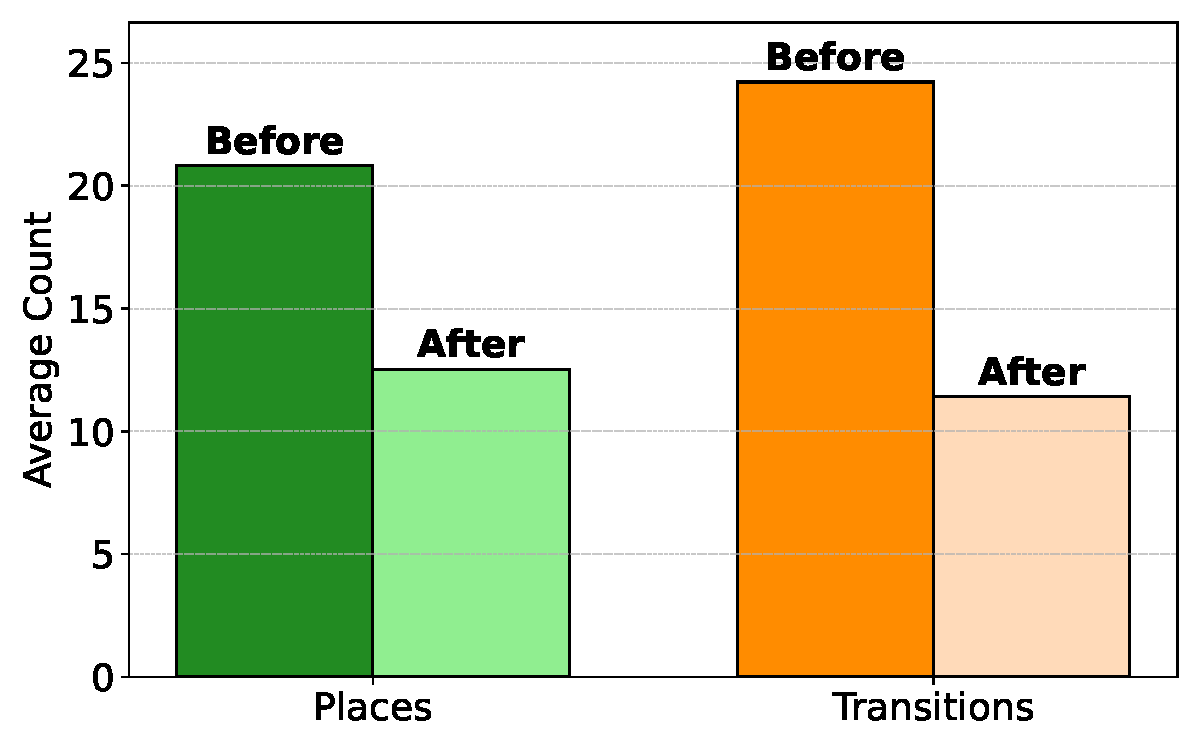
\includegraphics[width=0.4\textwidth]{plots/petri_size_reduction_plot.pdf}
	\caption{Size reduction of Petri nets through optimization techniques. The plot shows the reduction in the number of places and transitions after applying our optimization passes. Averaged on all Petri Nets of 50 benchmarks (timeout 30 seconds).}
	\label{fig:petri_size_reduction}
\end{figure}


	
\begin{tabular}{l c c c c}
	\toprule
	& \multicolumn{2}{c}{num components} & \multicolumn{2}{c}{periods per component} \\
	\cmidrule(lr){2-3} \cmidrule(lr){4-5}
	& mean & max & mean & max \\
	\midrule
	baseline (all optimizations)    &  3.28 (+0\%) &  22.00 (+0\%) & 1.36 (+0\%) &  4.00 (+0\%) \\
	baseline - remove\_redundant & 10.24 (+6.97\%) & 194 (+172\%)& \textbf{1.79 (+0.43\%)} & 11 (+7\%) \\
	baseline - generate\_less    &\textbf{782.38 (+779.10\%)}&\textbf{20484 (+20462\%)}&1.65 (+0.29\%)& \textbf{15 (+11\%)} \\
	baseline - smart\_order      &  3.36 (+0.09\%) &  22.00 (+0\%) & 1.38 (+0.02\%) &  4.00 (+0\%) \\
	\bottomrule
\end{tabular}
\textbf{The Table compares experiment running with a 30 second timeout}

\newpage